\documentclass[conference]{IEEEtran}
\IEEEoverridecommandlockouts
% The preceding line is only needed to identify funding in the first footnote. If that is unneeded, please comment it out.
\usepackage{cite}
\usepackage[lined,ruled,commentsnumbered,linesnumbered]{algorithm2e}
\usepackage{amsmath,amssymb,amsfonts}
\usepackage{algorithmic}
\usepackage{graphicx}
\usepackage{pdfpages}
\usepackage{subfigure}
\usepackage{textcomp}
\usepackage{xcolor}
\usepackage{subcaption}
\usepackage{verbatim}
\def\BibTeX{{\rm B\kern-.05em{\sc i\kern-.025em b}\kern-.08em
    T\kern-.1667em\lower.7ex\hbox{E}\kern-.125emX}}
\begin{document}

\title{Scheduling Multiple AI models in Optical Data Center Networks with a time-division multiplexing-based Multi-Stage Strategy\\
%{\footnotesize \textsuperscript{*}Note: Sub-titles are not captured in Xplore and
%should not be used}
%\thanks{Identify applicable funding agency here. If none, delete this.}
}

\author{\IEEEauthorblockN{Binjun Tang, Xiaoliang Chen and Zuqing Zhu\IEEEauthorrefmark{2}}
	\IEEEauthorblockA{School of Information Science and Technology, University of Science and Technology of China, Hefei, China \\
		\IEEEauthorrefmark{2}Email: \{zqzhu\}@ieee.org}}

\maketitle

%随着当前训练模型训练集和参数量大小的大幅提升,使用单个GPU训练模型会导致训练时间极长,内存资源无法容纳整个模型的参数等问题,分布式并行训练(如数据并行、专家并行等)被提出了以解决这些问题。随着GPU计算能力的提升和并行技术的成熟,模型训练的通信占比越来越高,训练瓶颈逐渐向通信转化。使用光数据中心网络训练大型分布式模型相较于传统使用电包交换的数据中心网络具有明显优势,被认为是当前大模型训练发展的方向。在我们以往的工作中研究了对光数据中心网络的业务调度,但是对业务的建模是粗糙的,而在这篇工作中,我们统一了不同业务的迭代模型,使得业务模型更加契合实际训练过程。并使用时分复用的方式设计了一种简单高效的双阶段业务调度方案,在一部分业务进行通信的时间进行另一部分业务的训练,从而大幅提示GPU利用率,间接提升模型训练效率。经过我们的仿真证明。。。。。。
\begin{abstract}
With the significant increase in the amount of parameters and the size of training datasets in current model training, single GPU can no longer accommodate the entire model's parameters, and the training time has become excessively long. This has led to the emergence of distributed parallel training methods, such as data parallelism (DP) and expert parallelism (EP). As GPU computation speed continues to improve, the proportion of communication in model training is increasing, which gradually shifting the training bottleneck towards communication. Utilizing optical data center networks (ODCN) for training large distributed models presents clear advantages over traditional electrical packet switch (EPS) data center networks, and is considered a promising direction for the development of large model training.

In our previous work, we explored job scheduling in ODCN, however, the modeling of jobs was somewhat rudimentary. In this paper, we reconstruct and refine the job models, creating a job model that aligns more closely with the actual training process. We also designed a simple yet efficient bi-stage job scheduling scheme using time division multiplexing method. This allows for the training of one set of jobs while another set is engaged in communication, significantly improving GPU utilization and, consequently, enhancing model training efficiency. Our simulations demonstrate that...
\end{abstract}

\begin{IEEEkeywords}
	ODCN, distributed training, parallelism, collective communication, time-division multiplexing, network schedule
\end{IEEEkeywords}

\section{Introduction}
%1. 随着AI的发展,大语言模型的参数量和训练集已经到达令人吃惊的规模,以GPT4为例,其参数量大小为1800B,训练数据集包含约13万亿个token。单个GPU的方案在做模型训练时会遇到训练时间极长,且内存无法容纳整个模型的问题,因此目前的AI训练常常在集群(如Meta、Colossus)中使用分布式训练方案,将模型和训练任务分摊给集群中的每个 GPU。随着单个 GPU 计算能力的提高,在集群中训练AI模型的速度提升日渐缓慢,GPU之间的通信延时占比越来越高逐渐成为训练过程中的瓶颈。如图1 所示,传统的数据中心网络用于训练集群中的模型时使用电路交换,这会导致pod间的带宽分配不够灵活,无法满足倾斜流量的需求,不仅如此,传统网络中采用ECMP协议,在训练时会出现哈希极化现象,这会大幅提高流量的倾斜度,并提高训练时间。而在图1(b)中的光数据中心网络中由于其可以灵活改变网络拓扑,从而适应不同倾斜方式的流量,且由于OXC一对一连接的性质,不会出现多条最优路径,因此更加适配集群中的AI模型训练。

With the advancement of artificial intelligence (AI), the scale of parameters and training dataset of large language model (LLM) have reached astonishing levels. For instance, GPT-4 boasts a parameter count of 1.8 trillion and is trained on a dataset comprising approximately 13 trillion tokens \cite{GPT4}. Single GPU solution encounters significant challenges during model training, including prolonged training times and insufficient memory to accommodate entire models. Consequently, current AI training often employs distributed training schemes \cite{surveyDML} within clusters (such as Meta \cite{Meta} and Colossus), distributing both models and training tasks across each GPU in the cluster. As the computational speed of individual GPU increases, the rate of improvement in training speed for AI models within clusters has gradually slowed, with communication latency between GPUs increasing in the proportion of iteration time and becoming a bottleneck in the training process. As illustrated in \emph{Figure} \ref{fig:sub1}, traditional data center networks utilize EPS for model training in clusters, resulting in inflexible bandwidth allocation between pods that fails to meet the demands of skewed traffic. Furthermore, the use of Equal-Cost Multi-Path (ECMP) protocol in traditional networks can lead to hash polarization during training \cite{HPN}, significantly increasing traffic skew and prolonging training times. In contrast, optical data center networks in \emph{Figure} \ref{fig:sub2} can flexibly adjust network topology to accommodate skewed traffic. Due to point-to-point connection characteristics of OXC, networks utilizing optical circuit switching (OCS) avoid the existence of multiple optimal paths, making them more suitable for AI model training within clusters.

%2. 在使用分布式方式训练模型时,需要将数据集和模型分配给每个GPU以并行训练,常用的并行方案有数据并行、专家并行等。在实际数据中心网络训练模型的过程中,常常会同时出现多种并行方案的训练任务。

When employing distributed methods for training models, it is necessary to allocate the dataset and model to each GPU for parallel training. Common parallelization strategies include data parallelism, expert parallelism. In practical data center networks, various parallel training tasks often occur simultaneously.

%在本文中,我们为多种并行方案业务的训练和通信过程进行了建模,并希望对这些业务进行统一调度。在光数据中心网络中分布式业务的调度相比传统数据中心网络更加复杂。由于ODCN中拓扑的重构延时较长,在百微秒级,因此重构时间和重构方案也是需要调度的,此时问题的复杂度会大幅提高。如果让所有业务在同一段时间内进行训练,在另一段时间进行计算,以此方式循环,此时我们可以很简单地获得调度放案。但是该方案计算和训练时间完全分开,网络的资源没有被完全使用,因此获得的方案结果往往并不好。为了迅速且高效地调度网络中的多种AI训练任务,我们提出了一种基于时分复用的四阶段算法,用于联合调度各业务的训练和通信过程。

In this paper, we model various parallel schemes for jobs and aim to achieve unified scheduling of these services.The scheduling of distributed jobs in ODCN is inherently more complex than in traditional data center networks. This complexity arises from the relatively long reconfiguration delay of the topology in ODCN, which can reach the order of hundreds of microseconds \cite{Zerwas2021}. Consequently, both the reconfiguration time and the reconfiguration schemes must be scheduled, significantly increasing the problem's complexity. Moreover, when considering the training process of individual jobs, we observe that during collective communication, the relevant GPUs remain idle and do not perform computations. This idleness leads to reduced GPU utilization, which indirectly impacts training efficiency. To address the need for rapid and efficient scheduling of multiple AI training jobs within the network, we propose a time-division multiplexing-based four-stage algorithm designed for the joint scheduling of training and communication processes across various jobs.

%这篇文章的贡献为:
The contribution of this paper is as follow:

\begin{itemize}
	%1.在ODCN中面向多种并行方案,对使用在网计算的业务结构进行系统建模;
	
	\item A systematic modeling of jobs utilizing INC is conducted with a focus on various parallel schemes in ODCN;
	
	%2.对这些业务提出了一种基于时分复用的双阶段策略,旨在以多项式时间复杂度内获得易于调度且高效的方案;
	
	\item A time-division multiplexing-based bi-stage strategy is proposed for these jobs, aiming to achieve an easily schedulable and efficient solution within polynomial time complexity.
	
	%3.经过我们的仿真证明,该方案相对于。。。。
	
	\item
\end{itemize}

\begin{figure}[htbp]
	\centering
	\begin{subfigure}
		\centering
		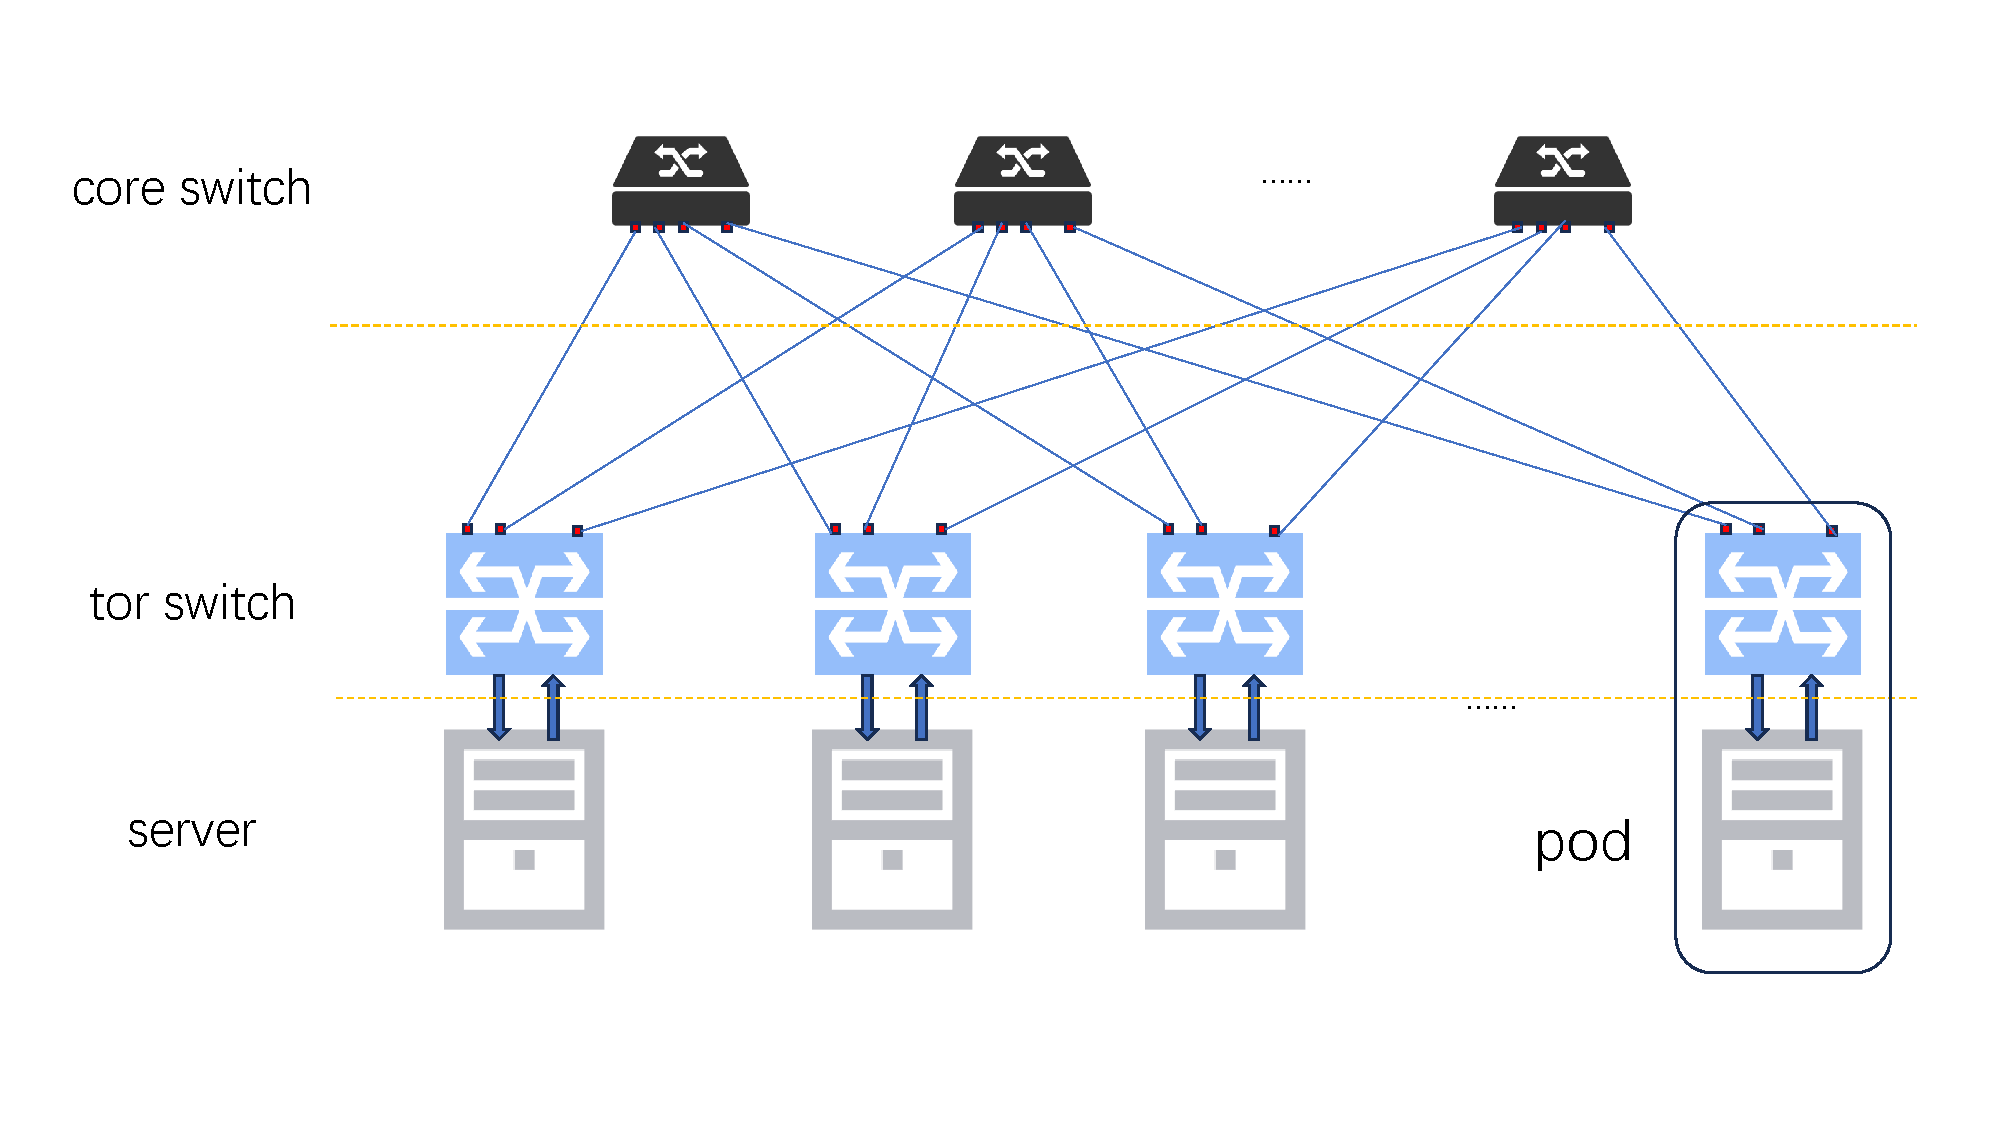
\includegraphics[width=\linewidth]{./figure/picture1.pdf}
		\caption{Traditional data center network}
		\label{fig:sub1}
	\end{subfigure}
	\begin{subfigure}
		\centering
		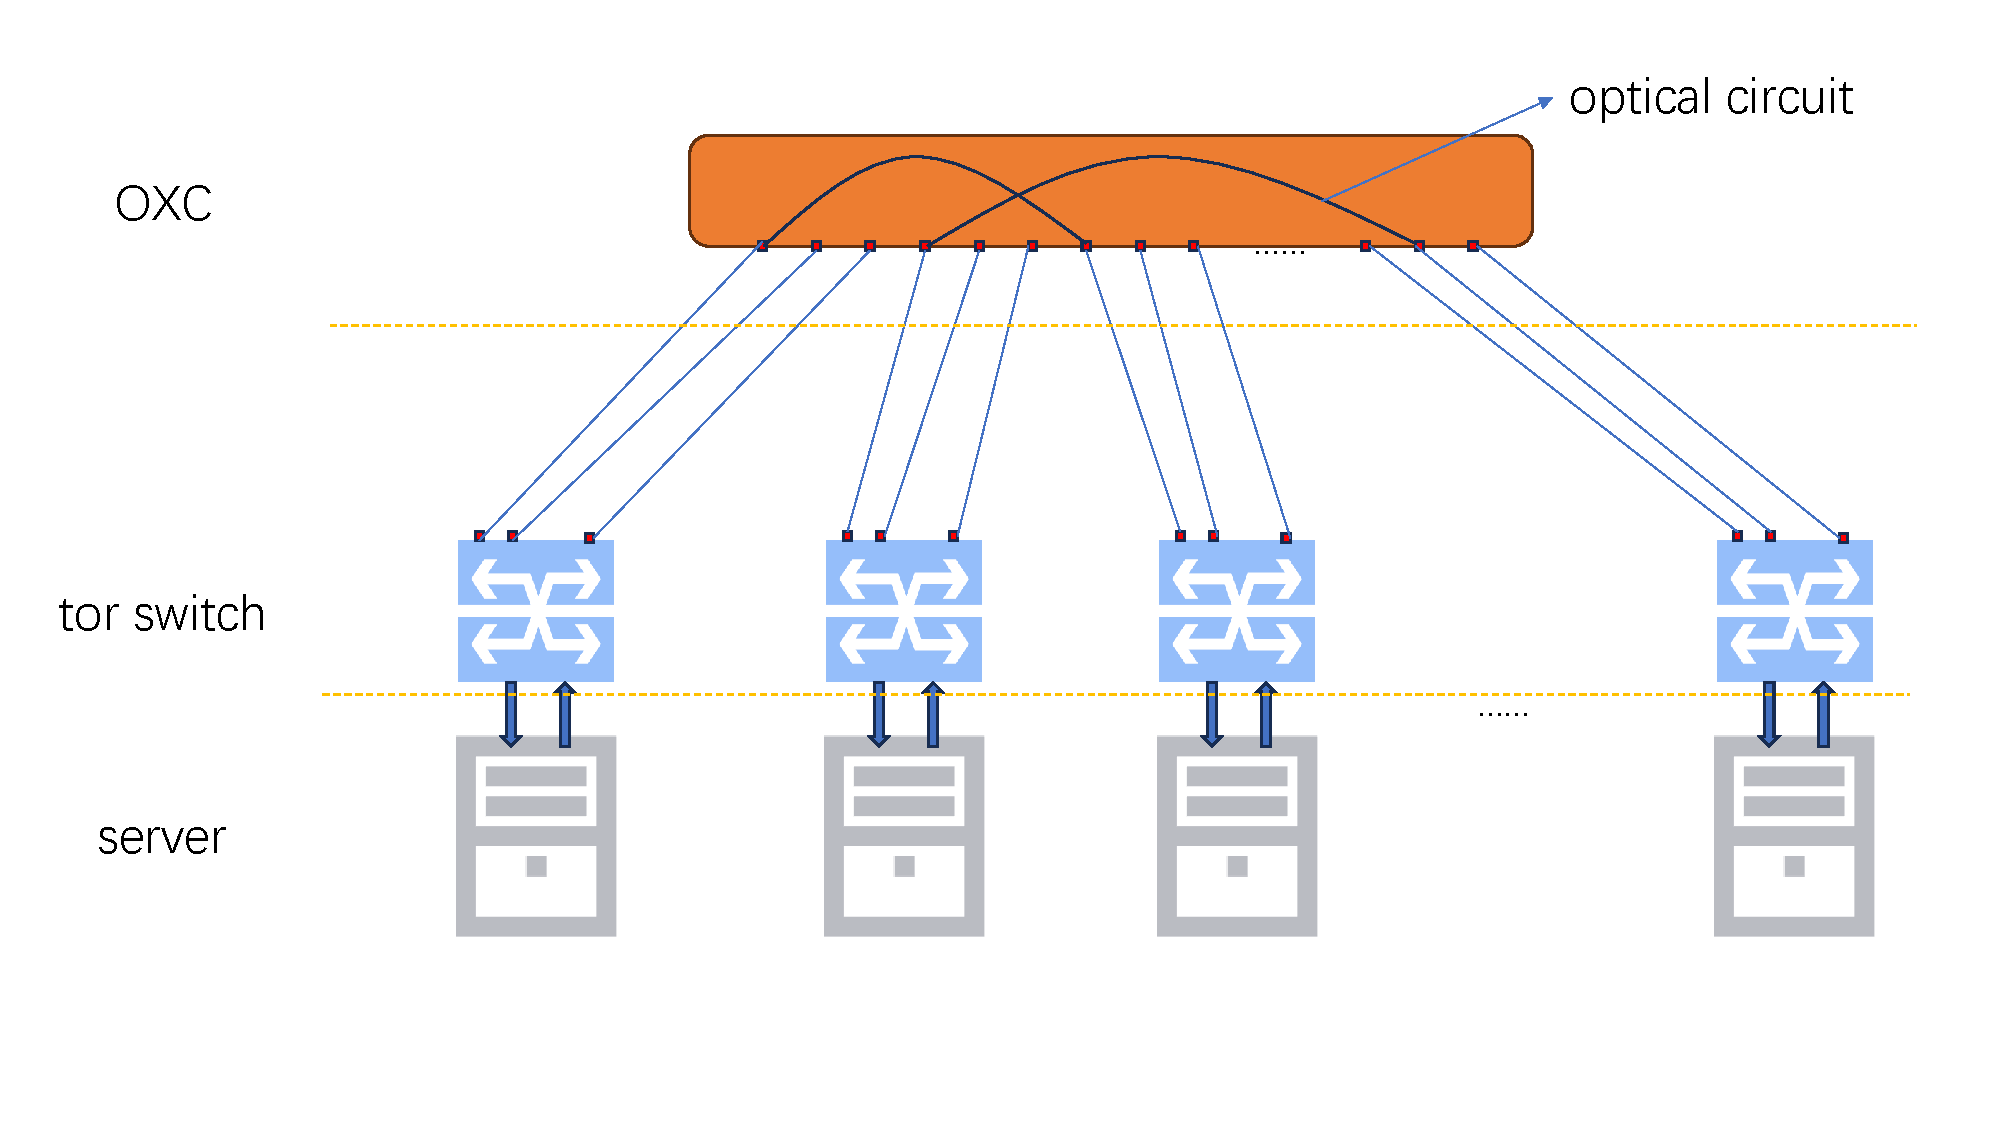
\includegraphics[width=\linewidth]{./figure/picture2.pdf}
		\caption{Optical data center network}
		\label{fig:sub2}
	\end{subfigure}
	\label{fig:total}
\end{figure}
\begin{figure}
	\centering
	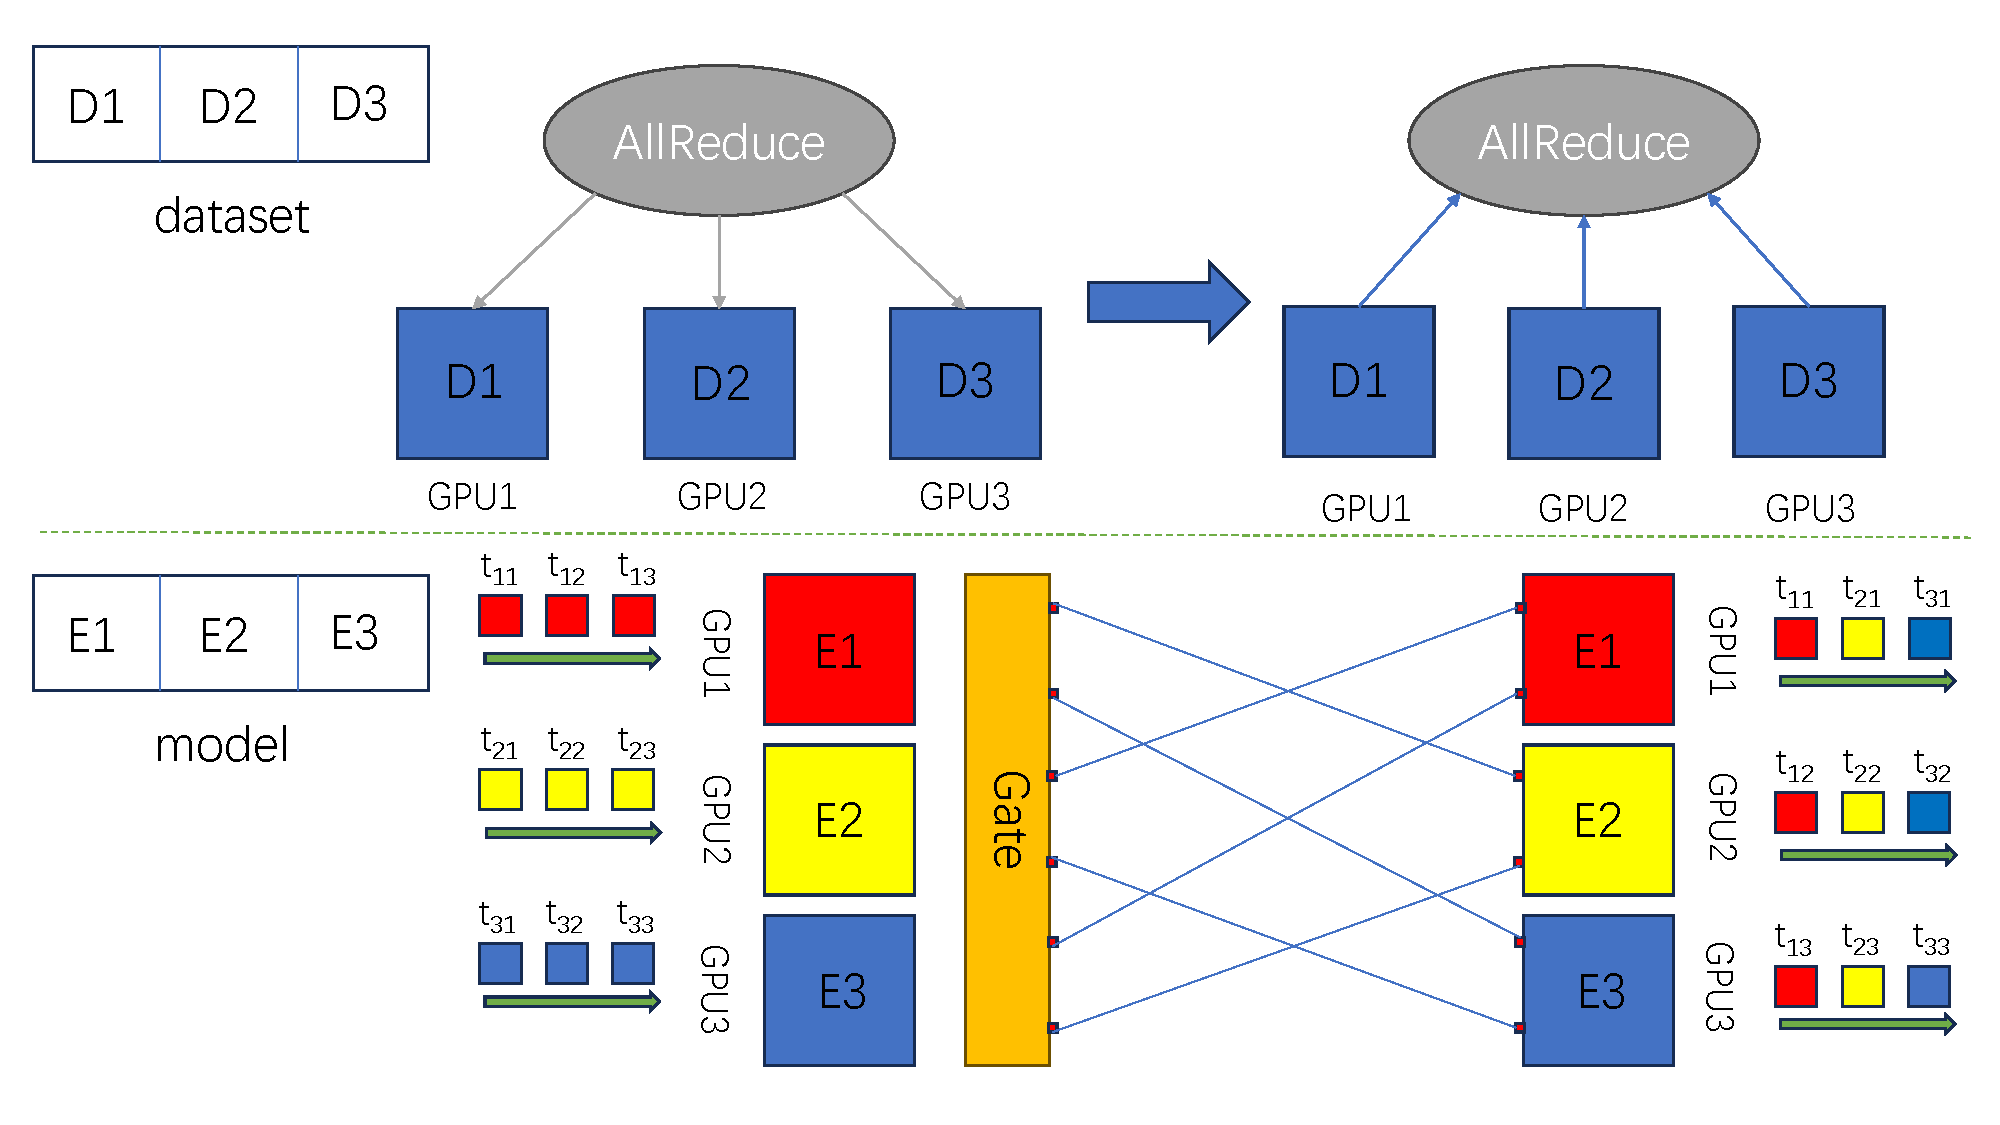
\includegraphics[width=1\linewidth]{figure/picture4}
	\caption{Training process of DP and EP}
	\label{fig:picture4}
\end{figure}

\begin{figure}
	\centering
	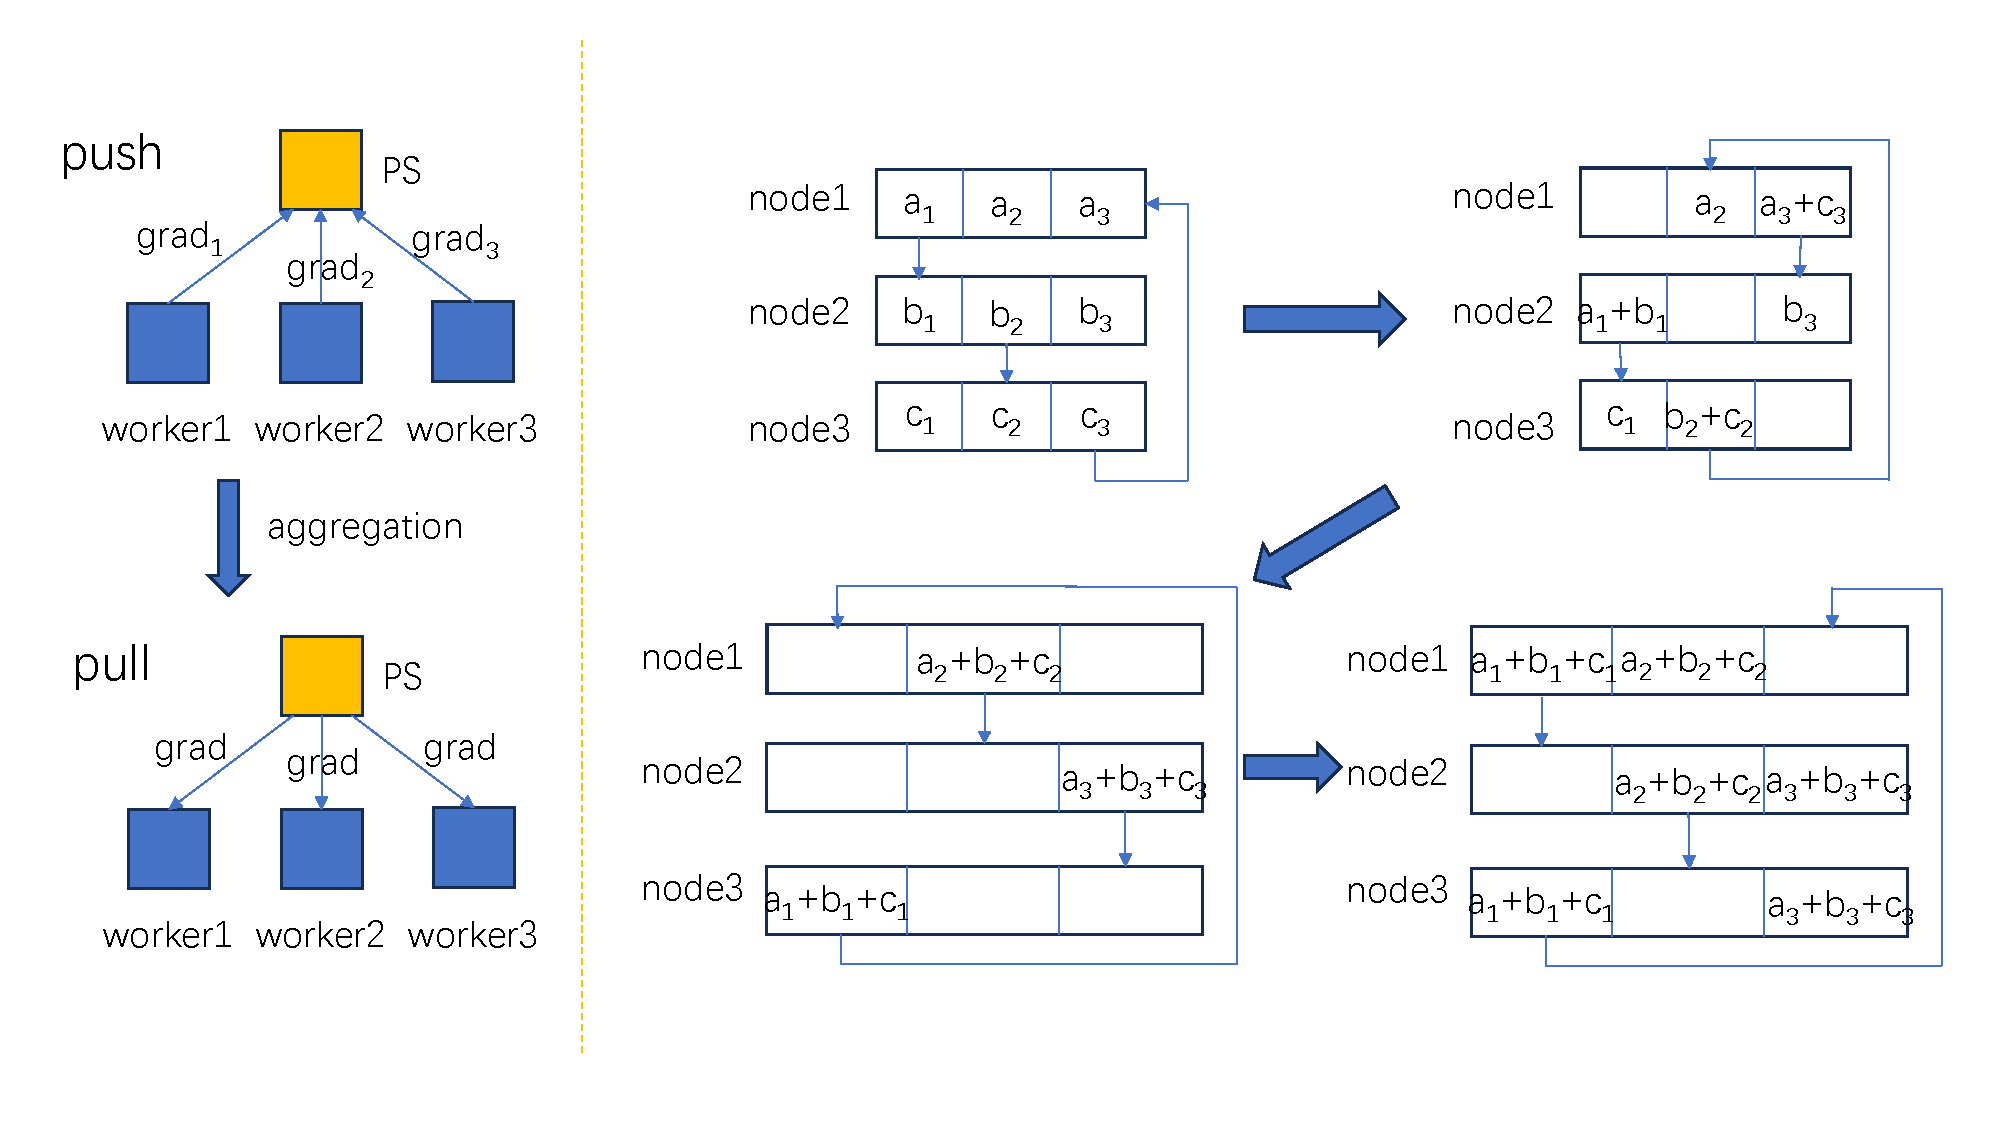
\includegraphics[width=1\linewidth]{figure/picture5}
	\caption{PS architecture and RAR architecture}
	\label{fig:picture5}
\end{figure}
\section{Problem Description}

\subsection{Network model}

%图1 (a) 表示了我们考虑的三层clos网络架构,主要由OXC层,ToR层和服务器层组成。OXC层用于完成ToR间的光互联通信,与包交换不同,OXC层在通信前需要提前在端口间建立一条一对一的连接,然后流量通过该连接从源端口进入目的端口。由于循环器的引入,OXC层的每条连接都是半双工通信,也就是说在同一时刻,一条连接只能提供一个方向的带宽。由于技术原因,OXC连接拓扑的重构延时在百微秒级,在模型训练时是无法忽视的。ToR层由每个pod的交换机组成,每个架顶交换机都连接了若干OXC端口用于与其他架顶交换机的通信。服务器层由若干pod下的GPU组成,用以执行训练任务。在通信需求产生后,流量会进入源所在pod对应的ToR,然后使用OXC将流量路由至目的pod对应的ToR。

\emph{Figure} \ref{fig:sub2} illustrates the three-layer Clos architecture under consideration, which primarily consists of the OXC layer, top-of-rack(ToR) layer, and server layer. The OXC layer is utilized to fulfill optical interconnect communication between ToRs. Unlike electrical packet switching, the OXC layer necessitates the establishment of a one-to-one connection between ports prior to communication, allowing traffic to flow from the source port to the destination port through this connection. With the introduction of circulators, each connection within the OXC layer enables full-duplex communication, meaning that a single connection can simultaneously provide bandwidth in both directions. Due to technical constraints, the reconfiguration delay of the OXC topology is on the order of hundreds of microseconds, which is a significant factor that cannot be overlooked during model training.The ToR layer consists of programmable ToR switches for each pod, with each switch connecting to several OXC ports for communication with other ToR switches. These switches are also capable of performing parameter aggregation for distributed training in place of parameter server. The server layer comprises GPUs in multiple pods for executing training tasks. Upon the generation of communication demands, traffic enters the ToR corresponding to the source pod and is then routed through the OXC to the ToR corresponding to the destination pod.

%我们使用两个平面来描述网络中的流量需求。由于pod内流量的存在,服务器层进入ToR的流量不一定会进入OXC。此时,使用OXC流量矩阵并不能完整描述流量状态,为了解决这一问题,我们使用了OXC平面和pod内平面来描述网络中的流量需求。OXC平面为双向无环图,使用$B_{oxc}^{i,j}$描述OXC层内从pod i到pod j的流量需求。pod内平面描述从ToR到相应pod内服务器的流量,使用$B_{in_pod}^i$来表示pod i中的这部分流量。因为集合通信的对称性,ToR到服务器的流量大小等于反向流量的大小。

We utilize two planes to characterize the traffic demand within the network. Due to the presence of intra-pod traffic and the utilization of INC, the traffic entering the ToR from the server layer does not necessarily flow into the OXC; similarly, the traffic transmitted to the ToR via the OXC connection may not enter the pod corresponding to this ToR. In this context, the OXC traffic matrix alone cannot comprehensively describe the traffic state. To address this issue, we employ the OXC plane and the intra-pod plane to represent the traffic demand in the network. The OXC plane is modeled as a bidirectional acyclic graph, with $B_{oxc}^{i,j}$ denoting the traffic demand from pod i to pod j within the OXC layer. The intra-pod plane describes the traffic from the ToR to the corresponding servers within the pod, represented by $B_{pod}^i$ for the traffic in pod i.Due to the symmetry of collective communication, the size of traffic from the ToR to the servers is equal to the size of traffic in the reverse direction.

\subsection{Job model}
%在本文中,我们考虑了三种集合通信类型的业务:PS类,Ring-AllReduce类和AllToAll类。前两种业务使用数据并行方案,AllToAll业务使用专家并行方案。

In this paper, we consider three types of collective communication workloads: PS type, RAR type, and AllToAll type. The first two types employ data parallelism, while the AllToAll type utilizes expert parallelism. 

\begin{itemize}
	% 数据并行:如图3上半部分表示,均分数据集,每个GPU存储了模型的所有参数,并训练属于它的一份数据集。在完成本轮训练后,需要使用随机梯度下降算法同步各GPU中的参数,然后使用同步后的参数进入下一轮的训练。在参数同步过程中,GPU间常用的集合通信方案有两种,分别为PS方案和AllReduce方案,这两种方案都兼容在网计算方式。在网计算可以使得网络中的交换机获得同步参数的能力,且在网计算与传输过程同时进行,也就是说在使用INC后,每一次迭代的聚合和通信过程是同步的。在数据中心网络中可以使用可编程交换机如Tofino,赋予架顶交换机在网计算能力。
	
	\item DP \cite{Parallelism}: As shown in the upper part of \emph{Figure} \ref{fig:picture4}, the dataset is evenly partitioned, with each GPU storing all parameters of the model and training its assigned subset of the dataset. After completing a training iteration, it is necessary to synchronize the parameters across the GPUs using the Stochastic Gradient Descent (SGD)  \cite{SGD2010} algorithm, after which the synchronized parameters are used for the subsequent training iteration. During the parameter synchronization process, two commonly utilized collective communication schemes between GPUs are the Parameter Server (PS) \cite{PS} scheme and the AllReduce scheme. PS and Ring-AllReduce (RAR) schemes are compatible with in-network computing (INC) \cite{INC2019, Rina}. INC enables the ability of switches within the network to synchronize parameters, allowing computation in switches and data transmission to occur simultaneously. In other words, with the implementation of INC, the aggregation and communication processes during each iteration are synchronized.	In data center networks, programmable top-of-rack (ToR) switches such as Tofino can be employed to enable the In-network computing ability of network.
	
	\begin{itemize}
		% PS:图四左边展示了PS架构怎样进行集合通信。使用参数服务器来同步各GPU间的参数,在各worker完成各自的训练后,将它们的参数传输给作为参数服务器的GPU,完成传输后在参数服务器上进行参数的聚合和更新,聚合后再将更新后的数据组播给各worker。
		\item PS: The left side of \emph{Figure} \ref{fig:picture5} illustrates how the PS architecture facilitates collective communication. The Parameter Server is employed to synchronize parameters among GPUs. After each worker completes its training process, the parameters are transmitted to the GPU designated as the Parameter Server. Following the completion of this transmission, parameter aggregation and updating occur on the Parameter Server. Subsequently, the updated data is multicast to all workers.
		
		% AllReduce:参数的聚合和更新操作本质上就是一种全规约,有多种算法可以实现AllReduce操作。其中,ring-AllReduce算法是目前最常用的方案,如图四所示,除此之外,双二叉树算法等也在集合通信库NCCL中被实现。
		\item AllReduce:Parameter aggregation and updating essentially represent an AllReduce operation, which can be realized through various algorithms without PS. Among these algorithms, the RAR algorithm is currently the most prevalent approach, as depicted in the right side of \emph{Figure} \ref{fig:picture5}. In addition, the double binary tree \cite{Tree} algorithm and others are also implemented within the collective communication library NCCL.
	\end{itemize}
	
	%专家并行:由于模型参数容量的爆炸式增长,单GPU已经无法存储大模型的所有参数。如图四右侧表示,专家并行将模型分为不同专家,各GPU存储一个专家的参数,训练数据根据其特征进入不同的专家。这种方案不仅可以大幅提升训练效率,还可以大幅降低单GPU参数存储量。与之相对的是它复杂的AllToAll集合通信需求,在每对专家之间都需要互相交换token以使其进入相应的专家。
	\item EP \cite{MoE}: Due to the explosive growth of model parameter capacity, single GPU can no longer accommodate all parameters of large models. As shown on the right side of \emph{Figure} \ref{fig:picture5}, expert parallelism addresses this challenge by partitioning the model into distinct experts, with each GPU storing the parameters of a specific expert. Training data is routed to different experts according to its characteristics. This approach not only significantly enhances training efficiency but also considerably reduces the parameter storage requirements for individual GPU. However, it introduces complex AllToAll collective communication demands, as tokens must be exchanged between every pair of experts to access to the according expert. 
\end{itemize}

\subsection{Time division multiplexing scheduling}

%无论业务的种类是什么,每次迭代都可以分成一次训练和一次通信,在业务的通信过程,其GPU处于空闲状态。我们提出了一种时分复用方式调度业务,也就是说,在一部分业务进行通信的过程,另一部分使用空闲的GPU进行训练。此时,通信中的业务空闲的GPU也被使用,大幅提高了GPU利用率,间接提高了训练效率。为了简化调度过程,我们将业务集合$J$分成A,B两组,在A组业务进行集体训练过程时,B组业务进行集体通信过程,我们将这个过程称为过程1,在两组全部完成后,B组业务使用A组业务的GPU进行训练,A组业务进行通信,这个过程为过程2,这两个过程使用不同的OXC拓扑,以适应不同的流量需求。将这两个过程合成一轮,整个调度过程由若干完全相同的轮组成。为了提高训练速度,我们选择以减少单轮用时
%$t_{round}$为优化目标,即$\min\{t_{round}\}$。我们通过调度业务的分组和GPU分配,并使用更高效的OXC拓扑来解决这一问题。

Regardless of the type of job, each iteration can be divided into a training phase and a communication phase, during which the GPUs are idle. We propose a time-division multiplexing scheduling approach, wherein one portion of the jobs undergoes communicating while another portion utilizes the idle GPUs for training. This effectively employs the idle GPUs during communication, significantly enhancing GPU utilization and indirectly improving training efficiency.To simplify the scheduling process, we classify the job set $J$ into two groups, A and B. While the A group engages in collective training, the B group conducts collective communication. We refer to this process as Process 1. Once both groups complete, the B group utilizes the GPUs from the A group for training, while the A group engages in communication; this is termed Process 2. These two processes utilize different OXC topology to accommodate varying traffic demands. The combination of these two processes constitutes a single round, and the entire scheduling process consists of several identical rounds. To enhance training speed, we aim to minimize the duration of a single round, denoted as $t_{round}$ , thus setting our optimization goal to $\min\{t_{round}\}$.We address this issue by scheduling the group and GPU allocation of jobs, while employing a more efficient OXC topology.

\subsection{ILP}

%为了严谨定量地描述刚才提出的问题,我们建立了一个整数线性规划模型。
\begin{equation}
	\min\{\sum_{t=1}^{2}\sum_{i=1}^{2}(t_{i,t})\}
\end{equation}

\begin{equation}
	\begin{split}
		\begin{cases}
			\begin{aligned}
				& t_{k, comm}^{t} = \max\{\dfrac{D^{k, t}_{i,j}}{B * L^k_{i,j}}, \dfrac{D_i^{k, t}}{B_{tor}}\}\\
				& D^{k, t}_{i,j} = \sum_{p\in group_{k, ps}}P^{p,t}_{i,j} + \sum_{r\in group_{k, ring}}R^{r}_{i,j} + \sum_{a\in group_{k,alltoall}}A^{a}_{i,j}\\
				& D^{k, t}_i = \sum_{p\in group_{k, ps}}P^{p,t}_{i} + \sum_{r\in group_{k, ring}}R^{r}_{i} + \sum_{a\in group_{k,alltoall}}A^{a}_{i}\\
			\end{aligned}
		\end{cases}\\
		\begin{aligned}
			, \forall i, j\in V, i \neq j, \forall k\in \{1,2\}\\
		\end{aligned}
	\end{split}
\end{equation}

\begin{equation}
	t_{k,t} = max\{t_{k, comm}^{t}, t_{train}^i\}, \forall i \in J/group_k, \forall t,k \in \{1,2\}
\end{equation}

\begin{equation}
	\begin{split}
		\begin{cases}
			\begin{aligned}
				& P_{i}^{p,t} = G_{i,p} * F_{p}, \forall p\in group_{k,ps}\\
				& R_{i}^{r} = 2 * G_{i,r} * F_{r}, \forall r\in group_{k,ring}\\
				& A_{i}^{a} = 2 * G_{i,a} * F_{a} * (U_{a} - 1), \forall a\in group_{k,alltoall}\\
			\end{aligned}
		\end{cases}\\
		\begin{aligned}
			,\forall i\in P,\forall t\in\{1,2\}
		\end{aligned}
	\end{split}
\end{equation}
\begin{equation}
	\begin{split}
		\begin{cases}
			\begin{aligned}
				& P_{i,n_p}^{p,1} = P_{n_p,i}^{p,2} = PN_i * F_i, \forall p \in group_{1,ps}\cup group_{2,ps}\\
				& R_{i,j}^{r} = Ring_{i,j} * F_i, \forall r \in group_{1,ring}\cup group_{2,ring}\\
				& A_{i,j}^a = AN_i * AN_j * F_i, \forall a \in group_{1,alltoall}\cup group_{2,alltoall}
			\end{aligned}
		\end{cases}\\
		\begin{aligned}
			,\forall i,j\in P,i\neq j
		\end{aligned}
	\end{split}
\end{equation}

\begin{equation}
	\begin{cases}
		\begin{aligned}
			& group_1 \cap group_2 = \emptyset \\
			& group_1 \cup group_2 = J \\
			& group_1 = group_{1,ps} \cup group_{1,ring} \cup group_{1, alltoall}\\
			& group_2 = group_{2,ps} \cup group_{2,ring} \cup group_{2, alltoall}
		\end{aligned}
	\end{cases}
\end{equation}

\section{Algorithm}
\subsection{Overall procedure}

%算法1展示了我们如何采用爬山法迭代求解最优分组。第一行使用公式***来估算每个业务单GPU训练用时,使用业务参数量来估计数据并行业务的通信量,专家并行业务使用batch size和单条数据 token 量估算通信量。第二行初始化A,B两组和邻域解集合NS。第三行到第十三行是爬山法迭代求解的过程,其中第四行到第八行表示迭代解替换为邻域内最优解。由于算法2中GPU资源被完全使用,在每个过程中如果通信时间更长,可以在不影响结果的情况下,按比例减少每个pod的GPU使用量。第九行使用迭代解找出所有邻域解。第十行使用算法2分别计算两个过程的OXC拓扑。第十一行计算两个组业务的训练时间。第十二行计算每个过程的用时,相加得到。

\emph{Algorithm} \ref{alg:Overall-algorithm} illustrates the iterative approach we employed using the hill-climbing method to determine the optimal solution. \emph{Line} 1 employs formula (1) to estimate the training time per GPU for each job. Here, K is a constant; specifically, K=8 when the model employs recomputation, and K=6 otherwise.$\Phi$ represents the quantity of model parameters.$F_{GPU}$ denotes the computational speed of the GPU.We can utilize the size of parameters to estimate the traffic size of data parallelism job, while expert parallelism job estimate their traffic size based on the number of tokens. \emph{Line} 2 initializes two groups, A and B, along with the neighborhood solution set NS. \emph{Line} 3 - 13 detail the iterative process of the hill-climbing method, where \emph{Line} 4-8 indicate the replacement of the iterative solution with the optimal solution from the neighborhood. Given that GPU resources are fully utilized in \emph{Algorithm} \ref{alg:count_topo}, if communication times are prolonged during each process, the GPU utilization for each pod can be proportionally reduced without affecting the results. \emph{Line} 9 identifies all neighborhood solutions using the iterative solution. \emph{Line} 10 calculates the OXC topology for both processes using \emph{Algorithm} \ref{alg:count_topo}. \emph{Line} 11 computes the training time for the jobs in both groups. Finally, \emph{Line} 12 adds the durations of each process to obtain $t_{round}$.

\begin{equation}
	t_{train} = \dfrac{K \times tokens \times \Phi}{F_{GPU} \times efficient}
\end{equation}

\begin{algorithm}
	\caption{Overall Procedure of Hill Climbing}
	\label{alg:Overall-algorithm}
	\LinesNumbered
	Predict the communication traffic $F_{oxc,k}^{i,j},F_{pod, k}^i$ of each workload and the iteration duration per GPU \;
	Initial group A = J,B = $\emptyset$, NS = $\emptyset$\;
	\While{$\max\{NS\} < t_{round}$ or NS = $\emptyset$}{
		\If{NS $\neq\emptyset$}{
			Modify the group A,B by the best neighborhood solution.\;
			$t_{round} = \max\{NS\}$\;
			Adjust GPU resource allocation based on communication duration.\;
		}
		Obtain a set of neighborhood solutions by exchanging the group of each workload.\;
		Apply \emph{Algorithm} \ref{alg:count_topo} to get OXC bandwidth $B_{oxc1}^{i,j},B_{oxc2}^{i,j}$ of the two processes\;
		Calculate training time of each group by $F_{oxc,k}^{i,j},F_{pod,k}^i,B_{oxc1}^{i,j},B_{oxc2}^{i,j},B_{pod}^i$\;
		Obtain $t_{round}$ of each neighborhood solutions and store them in $NS$\;
	}
	\textbf{Return} A, B, $t_{round}$ and corresponding OXC topology\;
\end{algorithm}

\subsection{Count OXC topology of each group}

% 算法2用来计算每一组的OXC拓扑。第一行预测每个业务的流量大小,然后降序排列至集合G中。第二行以用完网络中所有GPU和平均化业务训练时间的方式为每个业务确定GPU使用量。第三行初始化每个pod内ToR与服务器的流量和ToR与OXC的流量。第四到十九行为部署和连接拓扑的过程。其中第五到八行考虑当业务为PS型时,需要找一个OXC流量最低的pod作为ps。第九行对该业务初始化一个根节点集合用于后续组成环拓扑。第十行到第十五行按照部署流量最少pod上的原则,逐个部署业务的并行单元,如果不能把整个单元部署在该pod下,继续寻找下一个pod,直到该单元被完全部署,其中exc_rate指每个pod的OXC平面带宽与pod内平面带宽的比值。第十六到第十八行考虑业务为ring-AllReduce类时,需要调用算法3来确定成环方案。第二十行到二十一行,完成所有业务的部署后可以获得流量矩阵,并以此指导OXC拓扑的获得。

\emph{Algorithm} \ref{alg:count_topo} is utilized to compute the OXC topology for each group. \emph{Line} 1 predicts the traffic size of each job and puts them in descending order within set $G$. \emph{Line} 2 determines the GPU usage of each job by utilizing all GPUs in the network while averaging the training time of each job. \emph{Line} 3 initializes the traffic between ToR and servers, as well as the traffic between ToR and OXC within each pod. \emph{Line} 4 - 9 detail the process of deploying and connecting topology. Specifically, \emph{Line} 5 - 8 address the scenario where the job is of the PS type, requiring the identification of a pod with the lowest OXC traffic to serve as the PS. \emph{Line} 9 initializes a root node set for this service, which will be used to form a ring topology in subsequent steps. \emph{Line} 10 - 15 deploy the parallel units of the job sequentially, adhering to the principle of deploying on the pod with the minimum traffic. If a complete unit cannot be deployed on this pod, search for the next available pod until the entire unit is successfully deployed; here, exc\_rate represents the ratio of the OXC plane bandwidth to the intra-pod plane bandwidth for each pod. \emph{Line} 16 - 18 account for jobs of the ring-AllReduce type, apply \emph{Algorithm} \ref{alg:ring} to determine the ring formation scheme. Finally, \emph{Line} 20 - 21 indicate that upon completion of the deployment for all jobs, the traffic matrix can be obtained, which will subsequently guide the acquisition of the OXC topology.

\begin{algorithm}
	\caption{OXC topology algorithm of each group}
	\label{alg:count_topo}
	\LinesNumbered
	Predict the traffic size of each job and Sorting them in descending order in the set $G$.\;
	Utilizing all GPUs within the network and allocating GPU resources based on the average training duration.\;
	Initial tor\_traffic,oxc\_traffic = $[0]_{1\times|P|}$\;
	\For{each job k in set $G$}{
		\If{job k is PS type}{
			ps\_node = index of minimum oxc\_traffic\;
			update oxc\_traffic\;
		}
		root\_node = $\emptyset$\;
		\For{each parallelism unit of job k}{
			put $argmin_{p}\max\{\text{oxc\_traffic}_p, \dfrac{\text{tor\_traffic}_p}{\text{exc\_rate}}\}$ into root\_node\;
			\If{The unit cannot be fully placed in root pod}{
				Identify the next pod with the most abundant bandwidth and put remaining gpu until the unit is fully deployed\;
			}
		}
		\If{job k is RAR type}{
			Utilizing \emph{Algorithm} \ref{alg:ring} to form a ring connection among the root nodes\;
		}
	}
	Obtain traffic size $F_{i,j}$ of this group\;
	Determine the OXC topology $L_{i,j}$ by $F_{i,j}$\;
	\textbf{Return} OXC topology\;
\end{algorithm}

\subsection{How to form a ring}

%算法三考虑在业务使用环拓扑时如何成环,我们希望这个环拓扑可以与当前拓扑重复度更高,这样可以大幅降低拓扑复杂度,提高拓扑和流量矩阵的匹配度。第一行到第二行获得root\_node内节点对间已有连接的拓扑,并计算该拓扑内所有连接的节点度。要将这些节点连接成一个环,我们需要使得每个节点在拓扑中的节点度都为2,且不能存在子环。第三行到第八行控制所有节点度小于等于2,如果存在节点度大于2的节点,将找到这个节点节点度最大的零点,减去拓扑中这两个点的连接,直到root\_node中所有节点的节点度都不大于2。第九行找到所有互不相干的子拓扑,并剪断子环。第十行依次连接这些子拓扑,最终获得一个环拓扑,这个拓扑我们认为就是与当前拓扑重复度最高的。

\emph{Algorithm} \ref{alg:ring} addresses the formation of a ring topology when this job needs a ring topology. Our objective is to achieve a ring topology that exhibits a higher degree of redundancy with the current topology, thereby significantly reducing the complexity of the topology and enhancing the compatibility between OXC topology and traffic matrix.In \emph{Line} 1 - 2, we obtain the existing connections between node pairs within the root\_node and calculate the degrees of connectivity for all nodes in this topology. To connect these nodes into a ring, it is essential to ensure that each node has a degree of exactly 2 without forming any sub-rings. \emph{Line} 3 - 8 regulate the degrees of all nodes to be less than or equal to 2. If any node possesses a degree greater than 2, we identify the neighborhood with the highest degree and remove the connections between this node and this neighborhood in the topology, continuing this process until all nodes's degree in the root\_node are not greater than 2.In \emph{Line} 9, we identify all mutually disjoint sub-topologies and sever any sub-rings present. Finally, in \emph{Line} 10, we sequentially connect these sub-topologies to obtain a unified ring topology, which we consider to have the highest degree of redundancy with the current topology.

\begin{algorithm}
	\caption{Ring algorithm}
	\label{alg:ring}
	\LinesNumbered
	Initial Degree = $[0]_{0\times|P|}$\;
	Calculate Degree and link boolean value $L_{sub}^{i,j}$ in the sub-topology comprising only the root nodes.\;
	\For{each node n in root\_node}{
		\While{Degree\_n > 2}{
			Find the neighboring node $n'$ with the highest degree.\;
			$L_{sub}^{n,n'}=L_{sub}^{n',n} = 0$\;
		}
	}
	Identify all disjoint sub-topologies and severing the sub-rings\;
	Connect all sub-topologies sequentially and obtain a ring\;
	\textbf{Return} ring topology\;
\end{algorithm}

\section{Performance evaluations}
\begin{comment}
\subsection{Abbreviations and Acronyms}\label{AA}
Define abbreviations and acronyms the first time they are used in the text, 
even after they have been defined in the abstract. Abbreviations such as 
IEEE, SI, MKS, CGS, ac, dc, and rms do not have to be defined. Do not use 
abbreviations in the title or heads unless they are unavoidable.

\subsection{Units}
\begin{itemize}
\item Use either SI (MKS) or CGS as primary units. (SI units are encouraged.) English units may be used as secondary units (in parentheses). An exception would be the use of English units as identifiers in trade, such as ``3.5-inch disk drive''.
\item Avoid combining SI and CGS units, such as current in amperes and magnetic field in oersteds. This often leads to confusion because equations do not balance dimensionally. If you must use mixed units, clearly state the units for each quantity that you use in an equation.
\item Do not mix complete spellings and abbreviations of units: ``Wb/m\textsuperscript{2}'' or ``webers per square meter'', not ``webers/m\textsuperscript{2}''. Spell out units when they appear in text: ``. . . a few henries'', not ``. . . a few H''.
\item Use a zero before decimal points: ``0.25'', not ``.25''. Use ``cm\textsuperscript{3}'', not ``cc''.)
\end{itemize}

\subsection{Equations}
Number equations consecutively. To make your 
equations more compact, you may use the solidus (~/~), the exp function, or 
appropriate exponents. Italicize Roman symbols for quantities and variables, 
but not Greek symbols. Use a long dash rather than a hyphen for a minus 
sign. Punctuate equations with commas or periods when they are part of a 
sentence, as in:
\begin{equation}
a+b=\gamma\label{eq}
\end{equation}

Be sure that the 
symbols in your equation have been defined before or immediately following 
the equation. Use ``\eqref{eq}'', not ``Eq.~\eqref{eq}'' or ``equation \eqref{eq}'', except at 
the beginning of a sentence: ``Equation \eqref{eq} is . . .''

\subsection{\LaTeX-Specific Advice}

Please use ``soft'' (e.g., \verb|\eqref{Eq}|) cross references instead
of ``hard'' references (e.g., \verb|(1)|). That will make it possible
to combine sections, add equations, or change the order of figures or
citations without having to go through the file line by line.

Please don't use the \verb|{eqnarray}| equation environment. Use
\verb|{align}| or \verb|{IEEEeqnarray}| instead. The \verb|{eqnarray}|
environment leaves unsightly spaces around relation symbols.

Please note that the \verb|{subequations}| environment in {\LaTeX}
will increment the main equation counter even when there are no
equation numbers displayed. If you forget that, you might write an
article in which the equation numbers skip from (17) to (20), causing
the copy editors to wonder if you've discovered a new method of
counting.

{\BibTeX} does not work by magic. It doesn't get the bibliographic
data from thin air but from .bib files. If you use {\BibTeX} to produce a
bibliography you must send the .bib files. 

{\LaTeX} can't read your mind. If you assign the same label to a
subsubsection and a table, you might find that Table I has been cross
referenced as Table IV-B3. 

{\LaTeX} does not have precognitive abilities. If you put a
\verb|\label| command before the command that updates the counter it's
supposed to be using, the label will pick up the last counter to be
cross referenced instead. In particular, a \verb|\label| command
should not go before the caption of a figure or a table.

Do not use \verb|\nonumber| inside the \verb|{array}| environment. It
will not stop equation numbers inside \verb|{array}| (there won't be
any anyway) and it might stop a wanted equation number in the
surrounding equation.

\subsection{Some Common Mistakes}\label{SCM}
\begin{itemize}
\item The word ``data'' is plural, not singular.
\item The subscript for the permeability of vacuum $\mu_{0}$, and other common scientific constants, is zero with subscript formatting, not a lowercase letter ``o''.
\item In American English, commas, semicolons, periods, question and exclamation marks are located within quotation marks only when a complete thought or name is cited, such as a title or full quotation. When quotation marks are used, instead of a bold or italic typeface, to highlight a word or phrase, punctuation should appear outside of the quotation marks. A parenthetical phrase or statement at the end of a sentence is punctuated outside of the closing parenthesis (like this). (A parenthetical sentence is punctuated within the parentheses.)
\item A graph within a graph is an ``inset'', not an ``insert''. The word alternatively is preferred to the word ``alternately'' (unless you really mean something that alternates).
\item Do not use the word ``essentially'' to mean ``approximately'' or ``effectively''.
\item In your paper title, if the words ``that uses'' can accurately replace the word ``using'', capitalize the ``u''; if not, keep using lower-cased.
\item Be aware of the different meanings of the homophones ``affect'' and ``effect'', ``complement'' and ``compliment'', ``discreet'' and ``discrete'', ``principal'' and ``principle''.
\item Do not confuse ``imply'' and ``infer''.
\item The prefix ``non'' is not a word; it should be joined to the word it modifies, usually without a hyphen.
\item There is no period after the ``et'' in the Latin abbreviation ``et al.''.
\item The abbreviation ``i.e.'' means ``that is'', and the abbreviation ``e.g.'' means ``for example''.
\end{itemize}
An excellent style manual for science writers is \cite{b7}.

\subsection{Authors and Affiliations}
\textbf{The class file is designed for, but not limited to, six authors.} A 
minimum of one author is required for all conference articles. Author names 
should be listed starting from left to right and then moving down to the 
next line. This is the author sequence that will be used in future citations 
and by indexing services. Names should not be listed in columns nor group by 
affiliation. Please keep your affiliations as succinct as possible (for 
example, do not differentiate among departments of the same organization).

\subsection{Identify the Headings}
Headings, or heads, are organizational devices that guide the reader through 
your paper. There are two types: component heads and text heads.

Component heads identify the different components of your paper and are not 
topically subordinate to each other. Examples include Acknowledgments and 
References and, for these, the correct style to use is ``Heading 5''. Use 
``figure caption'' for your Figure captions, and ``table head'' for your 
table title. Run-in heads, such as ``Abstract'', will require you to apply a 
style (in this case, italic) in addition to the style provided by the drop 
down menu to differentiate the head from the text.

Text heads organize the topics on a relational, hierarchical basis. For 
example, the paper title is the primary text head because all subsequent 
material relates and elaborates on this one topic. If there are two or more 
sub-topics, the next level head (uppercase Roman numerals) should be used 
and, conversely, if there are not at least two sub-topics, then no subheads 
should be introduced.

\subsection{Figures and Tables}
\paragraph{Positioning Figures and Tables} Place figures and tables at the top and 
bottom of columns. Avoid placing them in the middle of columns. Large 
figures and tables may span across both columns. Figure captions should be 
below the figures; table heads should appear above the tables. Insert 
figures and tables after they are cited in the text. Use the abbreviation 
``Fig.~\ref{fig}'', even at the beginning of a sentence.

\begin{table}[htbp]
\caption{Table Type Styles}
\begin{center}
\begin{tabular}{|c|c|c|c|}
\hline
\textbf{Table}&\multicolumn{3}{|c|}{\textbf{Table Column Head}} \\
\cline{2-4} 
\textbf{Head} & \textbf{\textit{Table column subhead}}& \textbf{\textit{Subhead}}& \textbf{\textit{Subhead}} \\
\hline
copy& More table copy$^{\mathrm{a}}$& &  \\
\hline
\multicolumn{4}{l}{$^{\mathrm{a}}$Sample of a Table footnote.}
\end{tabular}
\label{tab1}
\end{center}
\end{table}
\begin{figure}[htbp]
\centerline{
\includegraphics{fig1.png}}
\caption{Example of a figure caption.}
\label{fig}
\end{figure}
Figure Labels: Use 8 point Times New Roman for Figure labels. Use words 
rather than symbols or abbreviations when writing Figure axis labels to 
avoid confusing the reader. As an example, write the quantity 
``Magnetization'', or ``Magnetization, M'', not just ``M''. If including 
units in the label, present them within parentheses. Do not label axes only 
with units. In the example, write ``Magnetization (A/m)'' or ``Magnetization 
\{A[m(1)]\}'', not just ``A/m''. Do not label axes with a ratio of 
quantities and units. For example, write ``Temperature (K)'', not 
``Temperature/K''.

\section*{Acknowledgment}

The preferred spelling of the word ``acknowledgment'' in America is without 
an ``e'' after the ``g''. Avoid the stilted expression ``one of us (R. B. 
G.) thanks $\ldots$''. Instead, try ``R. B. G. thanks$\ldots$''. Put sponsor 
acknowledgments in the unnumbered footnote on the first page.

\section*{References}

Please number citations consecutively within brackets \cite{b1}. The 
sentence punctuation follows the bracket \cite{b2}. Refer simply to the reference 
number, as in \cite{b3}---do not use ``Ref. \cite{b3}'' or ``reference \cite{b3}'' except at 
the beginning of a sentence: ``Reference \cite{b3} was the first $\ldots$''

Number footnotes separately in superscripts. Place the actual footnote at 
the bottom of the column in which it was cited. Do not put footnotes in the 
abstract or reference list. Use letters for table footnotes.

Unless there are six authors or more give all authors' names; do not use 
``et al.''. Papers that have not been published, even if they have been 
submitted for publication, should be cited as ``unpublished'' \cite{b4}. Papers 
that have been accepted for publication should be cited as ``in press'' \cite{b5}. 
Capitalize only the first word in a paper title, except for proper nouns and 
element symbols.

For papers published in translation journals, please give the English 
citation first, followed by the original foreign-language citation \cite{b6}.

\begin{thebibliography}{00}
\bibitem{b1} G. Eason, B. Noble, and I. N. Sneddon, ``On certain integrals of Lipschitz-Hankel type involving products of Bessel functions,'' Phil. Trans. Roy. Soc. London, vol. A247, pp. 529--551, April 1955.
\bibitem{b2} J. Clerk Maxwell, A Treatise on Electricity and Magnetism, 3rd ed., vol. 2. Oxford: Clarendon, 1892, pp.68--73.
\bibitem{b3} I. S. Jacobs and C. P. Bean, ``Fine particles, thin films and exchange anisotropy,'' in Magnetism, vol. III, G. T. Rado and H. Suhl, Eds. New York: Academic, 1963, pp. 271--350.
\bibitem{b4} K. Elissa, ``Title of paper if known,'' unpublished.
\bibitem{b5} R. Nicole, ``Title of paper with only first word capitalized,'' J. Name Stand. Abbrev., in press.
\bibitem{b6} Y. Yorozu, M. Hirano, K. Oka, and Y. Tagawa, ``Electron spectroscopy studies on magneto-optical media and plastic substrate interface,'' IEEE Transl. J. Magn. Japan, vol. 2, pp. 740--741, August 1987 [Digests 9th Annual Conf. Magnetics Japan, p. 301, 1982].
\bibitem{b7} M. Young, The Technical Writer's Handbook. Mill Valley, CA: University Science, 1989.
\end{thebibliography}
\vspace{12pt}
\color{red}
IEEE conference templates contain guidance text for composing and formatting conference papers. Please ensure that all template text is removed from your conference paper prior to submission to the conference. Failure to remove the template text from your paper may result in your paper not being published.
\end{comment}
\bibliographystyle{IEEEtran}
\bibliography{IEEEabrv, references}
\end{document}